\section{Análisis de la obra escultórica: Cristo de la Síndone de Miñarro} 

\begin{figure}[ht!]
    \centering
    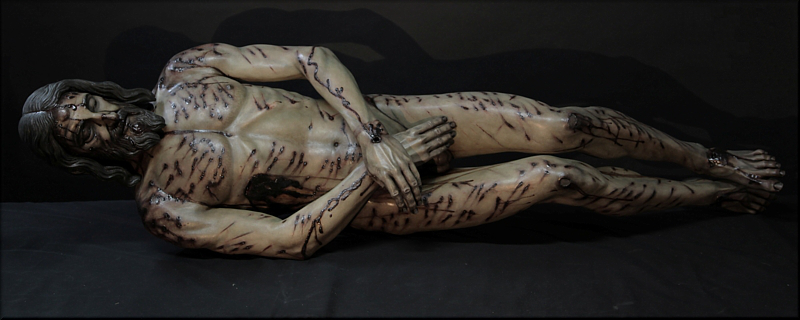
\includegraphics[width=1.0\textwidth]{minarro1.jpg}
    \caption{Cristo yacente de Miñarro: vista frontal. Copyright de www.lahornacina.com} %. URL: http://www.lahornacina.com/articulosminarro.htm
\end{figure}

\begin{figure}[ht!]
    \centering
    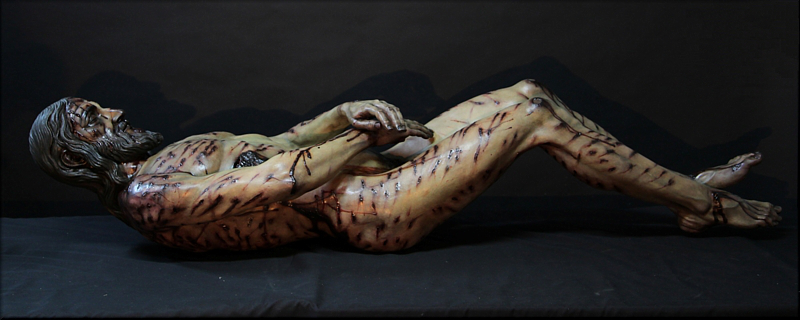
\includegraphics[width=1.0\textwidth]{minarro2.jpg}
    \caption{Cristo yacente de Miñarro: perfil. Copyright de www.lahornacina.com} %. URL: http://www.lahornacina.com/articulosminarro.htm
\end{figure}

\begin{figure}[ht!]
    \centering
    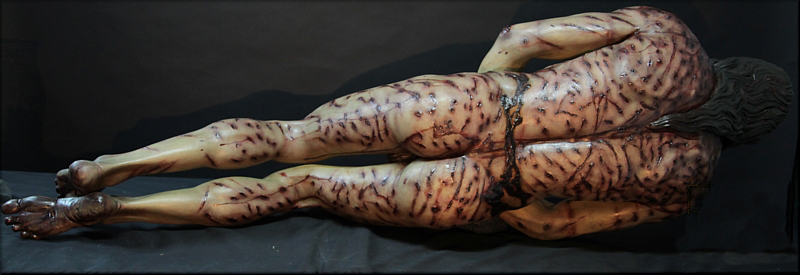
\includegraphics[width=1.0\textwidth]{minarro3.jpg}
    \caption{Cristo yacente de Miñarro: vista dorsal. Copyright de www.lahornacina.com} %. URL: http://www.lahornacina.com/articulosminarro.htm
\end{figure}

\newpage

\begin{description}
\item[Cronología:] 2012
\item[Lugar:] Exposición Sábana Santa (Itinerante)
\item[Estilo:] Realismo
%\item[Autor] Juan Manuel Miñarro
%\item[Título] Cristo de la Síndone o Sindónico
\end{description}

\textbf{Contexto histórico:} Esta obra es finalizada alrededor del año 2010, tras años empleados por el autor en su elaboración junto con otras esculturas que siguen la misma temática. Tanto es así, que existe otra figura de este mismo autor que reproduce el mismo Cristo pero en el momento de la crucifixión, en lugar de una vez fallecido (ver anexo\autoref{app:crucificadominarro}). El autor pretende mostrar lo más fielmente y científicamente posible la realidad de la muerte de Cristo. Se basa, por tanto, en una de las reliquias más conocidas, junto con el sudario de Oviedo, que posee relación con la muerte de Cristo: la Síndone de Turín o Sábana Santa (ver anexo\autoref{app:sindone}), realizando mediante el estudio meticuloso de ésta una impresionante escultura.

Aunque no está demostrado científicamente que la Síndone fuese la sábana que envolvió a Cristo tras su muerte, presenta ciertas características que han hecho que los expertos y estudiosos de todo el mundo la identifiquen como tal. Una característica que contribuye a ello es la propia imagen que conserva grabada, que por un lado posee las características propias de un hombre torturado y crucificado de la misma forma que Cristo según los evangelios, y que por otro lado se considera imposible de falsificar con las técnicas de las que se disponen hoy en día y más difícilmente aún en cualquier época anterior, puesto que es algo no se puede crear ni de forma natural ni de forma artificial.

En su búsqueda de la realidad el autor refleja de forma impecable las heridas, contusiones, laceraciones y demás aspectos que proveen a la obra de un dramatismo nunca visto hasta ahora en la muerte de Cristo ni en obras pictóricas ni escultóricas. Además plasma todos aquellos detalles que identifican a Cristo como un hombre torturado a la hora de su muerte.

\vspace{12pt}
\textbf{Anatomía de superficie:}

En esta obra se nos muestra a un Cristo muy estudiado desde absolutamente todas y cada una de las perspectivas desde las que se puede tener en cuenta: en su anatomía, en la reproducción de la muerte y en la representación de las heridas y contusiones.

Al centrarnos en el primer punto se puede observar una figura proporcionada, y anatómicamente coherente con el conocimiento anatómico actual y con la imagen de la Síndone, mediante la cual el autor ha logrado producir la silueta y los detalles de Cristo en su muerte de una forma realista. Se llega incluso a considerar la altura de Cristo sobre el metro ochenta, plasmando este aspecto también en la escultura.

Además, el autor refleja con gran detalle las lesiones de Cristo.

Podemos apreciar los hasta 120 latigazos de los que, supuestamente, fue víctima antes de ser crucificado y que están grabados con todo detalle en la piel de esta figura.

Los orificios provocados por los clavos pueden apreciarse en ambas muñecas, en la región carpiana, según la creencia actual, en lugar de en las palmas de las manos, entre los metacarpos. Y en los pies, que se cree que fueron clavados juntos con un solo clavo, debido a las características que presenta la Síndone, los orificios se encuentran en el punto de confluencia del calcáneo, astrágalo, escafoides y cuboides.

Igualmente se puede casi asegurar por la posición de los pies, el izquierdo flexionado unos noventa grados y el derecho extendido alrededor de ciento cincuenta y cinco grados, que el primero se encontraba sobre el segundo en el momento de la crucifixión.

En el rostro presenta un gran hematoma en el lado derecho, que se extiende desde debajo del arco cigomático hasta el ojo. Presenta también una rotura del tabique nasal. Ambas lesiones pudieron deberse a los puñetazos que le pegaron ante Caifás antes de ser condenado, o una bofetada según dice el evangelio de Juan (Jn 18, 22; Lc 22, 63; Mc 14, 65; Mt 26, 67), o incluso deberse a alguna caída en su recorrido al monte Calvario, ya que al llevar a cuestas el \textit{patibulum} no podría parar la caída con las extremidades superiores.

En la frente el autor nos muestra las heridas de la corona de espinas que continúan hacia la zona occipital de la cabeza, aunque son menos apreciables al estar cubiertas por el cabello.

No dejándose ningún detalle por el camino, el autor nos muestra las excoriaciones de las rodillas a la altura de la rótula, que podrían coincidir con las tres supuestas caídas de Cristo durante el camino al monte Calvario cargado con la cruz, que si bien no aparecen relatadas en la Biblia, sí que parecen obvias en la Síndone.

Así mismo el autor diferencia la proveniencia de la sangre, es decir, si Cristo todavía estaba vivo o si, por el contrario, ya estaba muerto cuando se produjo cada herida. Por ejemplo, en la herida del costado derecho producida por la lanza y situada por el autor entre la quinta y la sexta costilla, refleja el aspecto que podría tomar una herida postmortem, apreciándose la sangre como una masa coagulada y separada parcialmente del plasma, éste de un color más claro. La sangre proveniente de esta herida recorre, además, la zona lumbar de la espalda a modo de cinturón, como resultado del movimiento de Cristo de la cruz al sepulcro.

Claramente se trata de una figura que representa a Cristo muerto una vez producido el descendimiento de Cristo de la Cruz.

La figura mantiene una postura rígida provocada por el \textit{rigor mortis}, que se cree pudo empezar a originarse poco después de la muerte de Cristo, como ocurre en aquellas personas que han sido sometidas a grandes esfuerzos o actividad extenuante. De hecho es probable que el \textit{rigor mortis} comenzase cuando Cristo aún se encontraba suspendido en la cruz. Por ello podemos observar que las extremidades inferiores conservan la posición en la que estarían en ese momento.

Sin embargo la posición de los brazos no es la que tendría un crucificado que ha permanecido en la cruz durante el \textit{rigor mortis}: brazos casi completamente extendidos, en abducción y supinación del antebrazo, por lo que se asume que las extremidades superiores fueron forzadas antes de producirse el \textit{rigor mortis} completo, momento en el que la movilización de éstos habría sido imposible sin desgarrar tejidos. 

Otro detalle perteneciente a las extremidades superiores es que los primeros dedos de ambas manos se encuentran dispuestos sobre las palmas de las manos debido a una posible lesión del nervio mediano al introducir los clavos, aunque también podría ser la posición normal del primer dedo en la relajación muscular, que precede al \textit{rigor mortis}, por acción de los músculos flexores.

Debido a la contracción algunos músculos se aprecian más prominentes que en su estado habitual, es el caso de los músculos pectorales mayores, dando un aspecto de tórax distendido que contrasta con el vientre hundido de la figura, que hace posible la visión del borde costal inferior, así como parte de la caja torácica.

El crucificado muestra en las plantas de ambos pies un característico color azulado propio del \textit{livor mortis}. Éste consiste precisamente en la acumulación de la sangre por el efecto de la gravedad en las partes inferiores del cuerpo, según la posición de éste, proporcionando a la vez un color amarillento-ceniciento al resto del cuerpo por el que la sangre ya no fluye debido a la ausencia de latido cardíaco.

La figura estudiada demuestra que Cristo se mantuvo en la cruz después de muerto el tiempo suficiente como para que la sangre por efecto de la gravedad quedase retenida en la zona inferior de los miembros inferiores. Aunque no demasiado tiempo, pues en tal caso la cantidad de sangre acumulada en las extremidades inferiores sería superior, aun teniendo en cuenta la abundante sangre perdida antes y durante la crucifixión.

Además, queda patente que el cuerpo no ha permanecido en decúbito supino durante largo tiempo, ya que en tal caso la sangre también se habría acumulado en las zonas inferiores, en este caso la parte posterior de la figura.